\section{Empirical Evaluation}
\label{sec:evaluation}

\subsection{Research questions}

These seem quite pertinent to the overall problem of transparent science communication:
\begin{itemize}
\item How does performance degrade with partial/ambiguous information?
\item How is performance affected by ``adversarial'' (intentionally/unintentionally misleading) information?
\end{itemize}

Some ways we might explore these axes:
\begin{itemize}
\item meaningful vs.~meaningless vs.~misleading identifiers
\item leaving out key criteria (e.g.~year) that would resolve query to unique answer
\end{itemize}

We might want to distinguish ambiguity inherent in the problem domain (e.g.~uncertainty) vs.~ambiguity in the
specification of a particular code-generation query.

\subsection{Success Rate by Testcase}
To evaluate the system we used a sample of the Scigen dataset \cite{scigen_dataset_2021};
\label{subsec:success_rate_by_test_case}

\begin{figure}[!h]
    \centering
    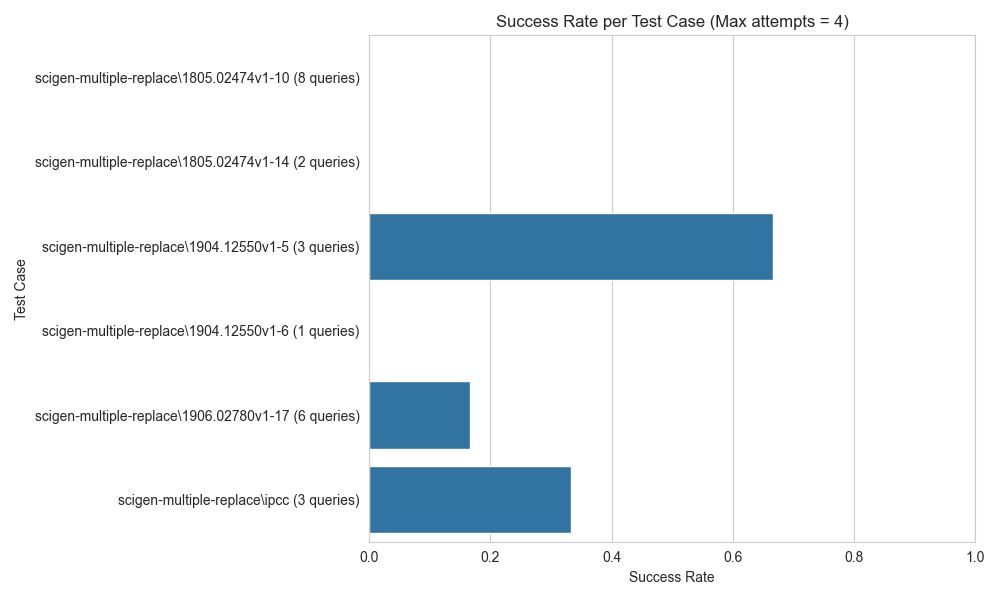
\includegraphics[width=0.95\linewidth]{fig/success_rate_by_test_case}
    \caption{Success rate by testcases}\label{fig:success_rate_by_test_case}
\end{figure}
